\begin{figure}[H]
\centering
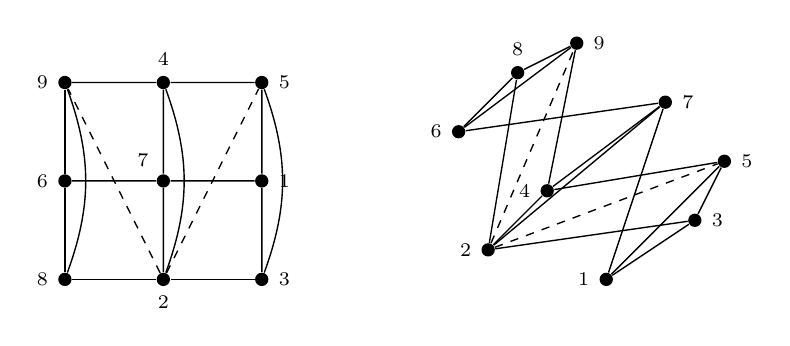
\begin{tikzpicture}[
  scale=1.25,
  vertex/.style={circle, fill=black, inner sep=1.7pt},
  edge/.style={line width=0.5pt}
]

% Left column: embedding
\begin{scope}[xshift=0cm]

  \node[vertex, label={[font=\scriptsize]left:9}] (4) at (0,2) {};
  \node[vertex, label={[font=\scriptsize]above:4}] (3) at (1,2) {};
  \node[vertex, label={[font=\scriptsize]right:5}] (8) at (2,2) {};

  \node[vertex, label={[font=\scriptsize]left:6}] (0) at (0,1) {};
  \node[vertex, label={[font=\scriptsize]above left:7}] (6) at (1,1) {};
  \node[vertex, label={[font=\scriptsize]right:1}] (5) at (2,1) {};

  \node[vertex, label={[font=\scriptsize]left:8}] (2) at (0,0) {};
  \node[vertex, label={[font=\scriptsize]below:2}] (1) at (1,0) {};
  \node[vertex, label={[font=\scriptsize]right:3}] (7) at (2,0) {};

  \draw[edge] (0) -- (2);
  \draw[edge] (0) -- (4);
  \draw[edge] (0) -- (6);
  
  \draw[edge] (1) -- (2);
  \draw[edge] (1) to[bend right=20] (3);
  \draw[edge, dashed] (1) -- (4);
  \draw[edge] (1) -- (6);
  \draw[edge] (1) -- (7);
  \draw[edge, dashed] (1) -- (8);
  
  \draw[edge] (2) to[bend right=20] (4);
  
  \draw[edge] (3) -- (4);
  \draw[edge] (3) -- (6);
  \draw[edge] (3) -- (8);
  
  \draw[edge] (5) -- (6);
  \draw[edge] (5) -- (7);
  \draw[edge] (5) -- (8);
  
  \draw[edge] (7) to[bend right=20] (8);
\end{scope}

% Right column: comparability graph
\begin{scope}[xshift=4cm,yscale=1,scale=0.3]
\node[vertex, label={[font=\scriptsize]left:6}] (0) at (0,5) {};
\node[vertex, label={[font=\scriptsize]left:2}] (1) at (1,1) {};
\node[vertex, label={[font=\scriptsize]above:8}] (2) at (2,7) {};
\node[vertex, label={[font=\scriptsize]left:4}]  (3) at (3,3) {};
\node[vertex, label={[font=\scriptsize]right:9}] (4) at (4,8) {};
\node[vertex, label={[font=\scriptsize]left:1}]  (5) at (5,0) {};
\node[vertex, label={[font=\scriptsize]right:7}] (6) at (7,6) {};
\node[vertex, label={[font=\scriptsize]right:3}]  (7) at (8,2) {};
\node[vertex, label={[font=\scriptsize]right:5}]  (8) at (9,4) {};

\draw[edge] (0) -- (2);
\draw[edge] (0) -- (4);
\draw[edge] (0) -- (6);

\draw[edge] (1) -- (2);
\draw[edge] (1) -- (3);
\draw[edge,dashed] (1) -- (4);
\draw[edge] (1) -- (6);
\draw[edge] (1) -- (7);
\draw[edge,dashed] (1) -- (8);

\draw[edge] (2) -- (4);

\draw[edge] (3) -- (4);
\draw[edge] (3) -- (6);
\draw[edge] (3) -- (8);

\draw[edge] (5) -- (6);
\draw[edge] (5) -- (7);
\draw[edge] (5) -- (8);

\draw[edge] (7) -- (8);
\end{scope}
\end{tikzpicture}
\caption{The width 3 graph gadget viewed as a grid with additional edges (left) and as a subgraph of $\CGrid$ (right).}
\label{fig:width-3-gadget}
\end{figure}